% $Id: template.tex 11 2007-04-03 22:25:53Z jpeltier $

%\documentclass{vgtc}                          % final (conference style)
%\documentclass[review]{vgtc}                 % review
%\documentclass[widereview]{vgtc}             % wide-spaced review
%\documentclass[preprint]{vgtc}               % preprint
\documentclass[electronic]{vgtc}             % electronic version

%% Uncomment one of the lines above depending on where your paper is
%% in the conference process. ``review'' and ``widereview'' are for review
%% submission, ``preprint'' is for pre-publication, and the final version
%% doesn't use a specific qualifier. Further, ``electronic'' includes
%% hyperreferences for more convenient online viewing.

%% Please use one of the ``review'' options in combination with the
%% assigned online id (see below) ONLY if your paper uses a double blind
%% review process. Some conferences, like IEEE Vis and InfoVis, have NOT
%% in the past.

%% Figures should be in CMYK or Grey scale format, otherwise, colour 
%% shifting may occur during the printing process.

%% These few lines make a distinction between latex and pdflatex calls and they
%% bring in essential packages for graphics and font handling.
%% Note that due to the \DeclareGraphicsExtensions{} call it is no longer necessary
%% to provide the the path and extension of a graphics file:
%% \includegraphics{diamondrule} is completely sufficient.
%%
\ifpdf%                                % if we use pdflatex
  \pdfoutput=1\relax                   % create PDFs from pdfLaTeX
  \pdfcompresslevel=9                  % PDF Compression
  \pdfoptionpdfminorversion=7          % create PDF 1.7
  \ExecuteOptions{pdftex}
  \usepackage{graphicx}                % allow us to embed graphics files
  \DeclareGraphicsExtensions{.pdf,.png,.jpg,.jpeg} % for pdflatex we expect .pdf, .png, or .jpg files
\else%                                 % else we use pure latex
  \ExecuteOptions{dvips}
  \usepackage{graphicx}                % allow us to embed graphics files
  \DeclareGraphicsExtensions{.eps}     % for pure latex we expect eps files
\fi%

%% it is recomended to use ``\autoref{sec:bla}'' instead of ``Fig.~\ref{sec:bla}''
\graphicspath{{figures/}{pictures/}{images/}{./}} % where to search for the images

\usepackage{microtype}                 % use micro-typography (slightly more compact, better to read)
\PassOptionsToPackage{warn}{textcomp}  % to address font issues with \textrightarrow
\usepackage{textcomp}                  % use better special symbols
\usepackage{mathptmx}                  % use matching math font
\usepackage{times}                     % we use Times as the main font
\renewcommand*\ttdefault{txtt}         % a nicer typewriter font
\usepackage{cite}                      % needed to automatically sort the references
\usepackage{tabu}                      % only used for the table example
\usepackage{booktabs}                  % only used for the table example
%% We encourage the use of mathptmx for consistent usage of times font
%% throughout the proceedings. However, if you encounter conflicts
%% with other math-related packages, you may want to disable it.


%% If you are submitting a paper to a conference for review with a double
%% blind reviewing process, please replace the value ``0'' below with your
%% OnlineID. Otherwise, you may safely leave it at ``0''.
\onlineid{0}

%% declare the category of your paper, only shown in review mode
\vgtccategory{Summary}

%% allow for this line if you want the electronic option to work properly
\vgtcinsertpkg

%% In preprint mode you may define your own headline.
%\preprinttext{To appear in an IEEE VGTC sponsored conference.}

%% Paper title.

\title{Survey: Visual Analysis Approaches to Time Series Prediction}

%% This is how authors are specified in the conference style

%% Author and Affiliation (single author).
\author{Fabian Otto\thanks{e-mail: fabian.otto@stud.tu-darmstadt.de}}
\affiliation{\scriptsize Technical University Darmstadt}

%% A teaser figure can be included as follows, but is not recommended since
%% the space is now taken up by a full width abstract.
%\teaser{
%  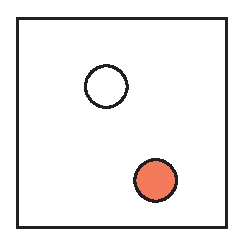
\includegraphics[width=1.5in]{sample.eps}
%  \caption{Lookit! Lookit!}
%}

%% Abstract section.
\abstract{
	
} % end of abstract

% \nocopyrightspace

%%%%%%%%%%%%%%%%%%%%%%%%%%%%%%%%%%%%%%%%%%%%%%%%%%%%%%%%%%%%%%%%
%%%%%%%%%%%%%%%%%%%%%% START OF THE PAPER %%%%%%%%%%%%%%%%%%%%%%
%%%%%%%%%%%%%%%%%%%%%%%%%%%%%%%%%%%%%%%%%%%%%%%%%%%%%%%%%%%%%%%%%

\begin{document}

\firstsection{Introduction}

\maketitle

% TODO rewrite
%TS3 introduction 
Predictive analytics is concerned with the prediction of future probabilities and trends based on observed events. 
It encompasses a multi-perspective approach that includes integrated reasoning, pattern recognition and predictive modeling associated with domain knowledge.
However, the primary use of such systems tends to be reactive, meaning that analytic systems are typically.

The increasing availability of digital data provides both opportunities and challenges.
The potential of utilizing these data for increasing effectiveness and efficiency of operations and decision making is vast. 
Harnessing this data with effective tools can transform decision making from reactive to proactive and predictive. 
However, the volume, variety, and velocity of these data can actually decrease the effectiveness of analysts and decision makers by creating cognitive overload and paralysis by analysis, especially in fast-paced decision making environments.

% spatial
In spatiotemporal data, analysts are searching for regions of space and time with unusually high incidences of events.
In the cases that hotspots are found, analysts would like to predict how these regions may grow in order to plan decision support and preventative measures.
Furthermore, analysts would also like to predict where future hotspots may occur.

Four stages:
\begin{enumerate}
	\item data cleaning, 
	\item feature selection, 
	\item modeling, 
	\item and validation
	
\end{enumerate}

\section{Temporal Time Series \label{sec:temporal}}
content 
\subsection{Simple Time Series (maybe just use \autoref{subsec:pattern}, check what makes more sense)\label{subsec:simple}}
\subsection{Pattern and Anomaly Detection\label{subsec:pattern}}
The easiest kind of prediction can be found with simple time series, they are only based on a single variable and include one single history. 

TS is also multivariate.




An early work with simple time series can be found from Buono et al. \cite{buono:2005}.
They built upon the TimeSearcher system proposed by Hochheiser and Shneiderman \cite{Hochheiser:2004}, which focuses explicitly on high usability even for users without specialized skills such as statistics.
% and implemented a second  and third version \cite{buono:2007}.
Based on their idea, Buono et al. continued with using timeboxes, i.e. rectangular regions that filter the data and reduce the scope of each search.
Their updated version, extends the original timeboxes with another variant for pattern search in the remaining data. 
Further, they also allow users to work with long time series of multiple heterogeneous variables. 
For data exploration the user is initially presented with a multivariable time series viewer, which allows to visually analyze multiple variables in parallel in different levels of detail.
In order to detect pattern, the systems allows the user to highlight a pattern within the time series to search for. 
Therefor, the search space can be limited to only interesting areas.
The initial matches of the given pattern can afterwards be refined to support the goal better. 
This process of returning many results and consequently enable the user to reduce the outcome to his/her liking, can also be found in spatiotemporal approaches (see \autoref{sec:spatiotemp}), esp. in the template driven approach of \cite{malik:2014}.
Moreover, TimeSearcher also provides different data transformations to match patterns more easily. 
One drawback of the system is that it cannot deal with missing data points and pattern matching still remains very depended on the user chosen parameters.

This second version of TimeSearcher was updated once more by Buono et al. \cite{buono:2007}.
It focuses mainly on a similarity-based data-driven forecast, which uses line charts for visualization.
To avoid the overlapping issue for an increasing number of items, the system offers a summarized view based on a river plot, which also displays a confidence bands.
This data-driven approach extrapolates the time series based on a similarity search of past events to predict future events. 
As in \cite{buono:2005} the system is meant for users without statistical knowledge.
For that reason, a simultaneous preview interface allows to compare multiple parameter choices in parallel. 
Given those ideas, some drawbacks of have to be considered as well. 
Data-driven approaches normally require larger datasets compared to a model-driven approach.
Furthermore, the system's prediction output still relies heavily on the choices of an untrained user.

Another extension of an existing system is from B{\"o}gel et al. \cite{boegel:2013}, who built a prediction functionality on top of their earlier work \cite{boegel:2013}.
Unlike \cite{Hochheiser:2004, buono:2005, buono:2007} the system is model-driven, and therefore it requires less data points.
Originally, the system was designed after the Box Jenkins method \cite{box:1976} and meant for model selection, however, during their evaluation, they found that an actual prediction functionality would also improve the model selection process.
While being able to adjust different model parameters (e.g. for Autoregressive, Moving Average or Autoregressive integrated moving average models), the prediction visualizations are changing in parallel. 
As visualizations, the system provides, similar to \cite{buono:2007}, line charts with corresponding confidence bands.
Additionally, they specifically visualize the difference of true and predicted values for each data point as well as the direction (positive or negative).
This gives the analyst a quick overview if the model is constantly over- or underestimating the time series and how long and often this occurs.

Another system can be found from Steed et al. \cite{steed:2017}.
Their approach is focused on understanding patterns in log and imagery data collected by 3D printers.

%\begin{figure}[tb]
% \centering
% 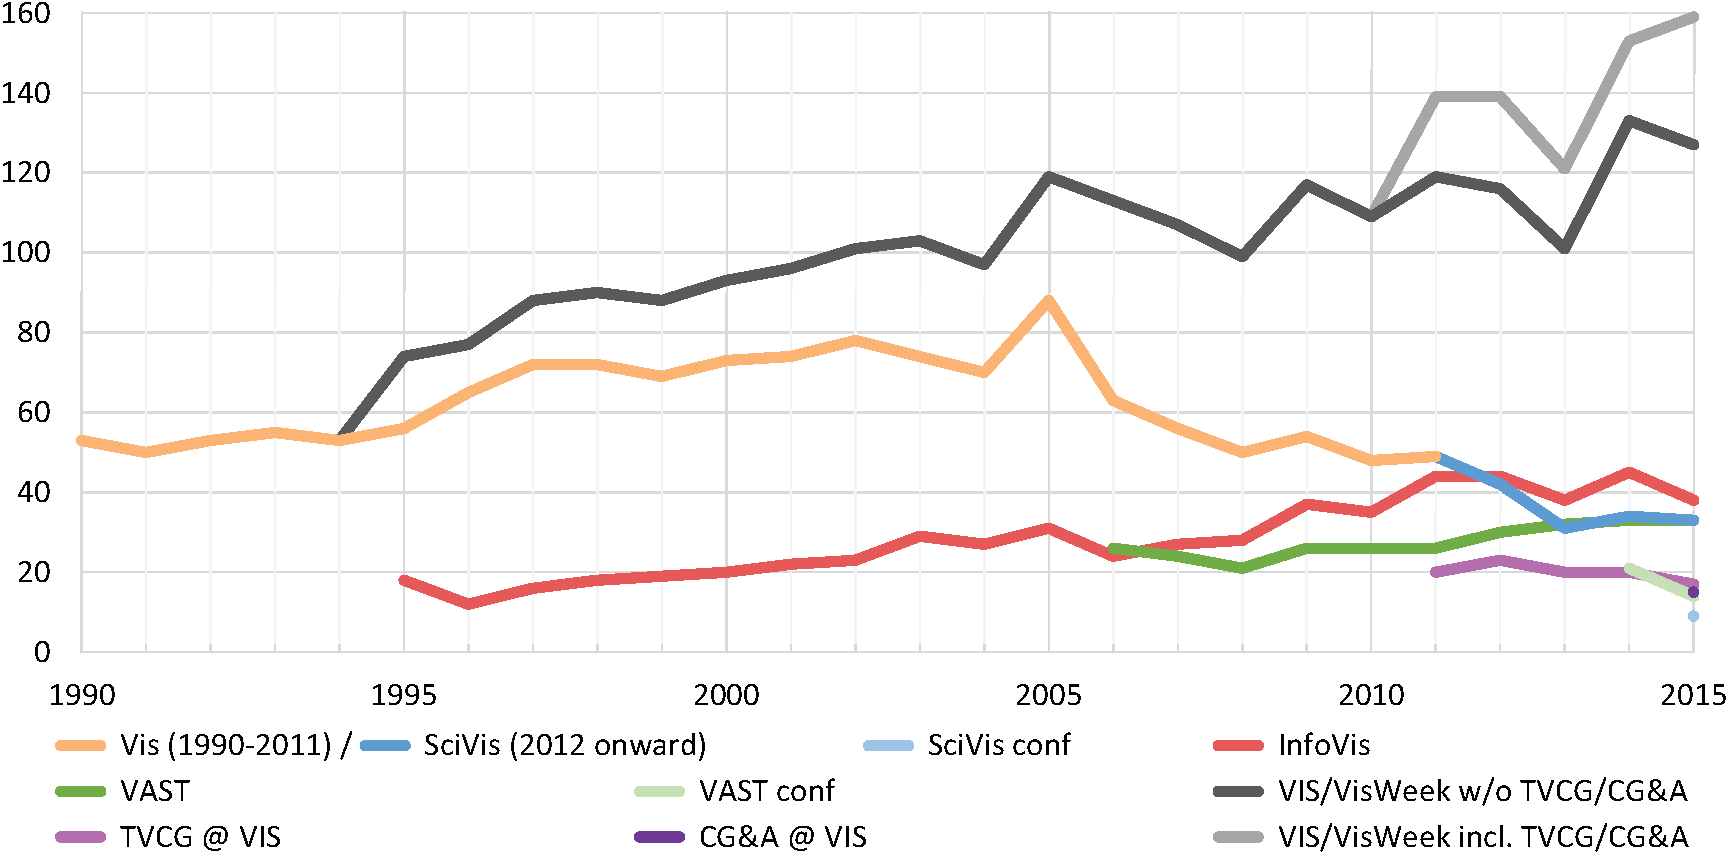
\includegraphics[width=\columnwidth]{paper-count-w-2015-new}
% \caption{A visualization of the 1990--2015 data from . The image is from and is in the public domain.}
% \label{fig:sample}
%\end{figure}


\subsection{Time Series Prediction with Peak Preservation \label{subsec:peak}}
content

\subsection{Multivariate Time Series \label{subsec:multivar}}
Visual Analytics approaches for simple time series prediction (\autoref{subsec:simple}) offer a great variety for single time series.
However, in a practical environment it is often necessary to evaluate multiple time series in parallel or deal with multidimensional input variables.
In order to solve these problems, visual analytics approaches for simple time series are not sufficient anymore.\\ 
An older Visual Analytics approaches for multivariate time series prediction is from Ichikawa et al. \cite{ichikawa:2002}.
Their goal was to predict multiple daytime stock prices and simultaneously visualize a set of prediction from different simulation systems within a single system. 
Therefor, their system supports multiple prediction for a single stock as well as predictions of multiple stocks. 
One major finding was, visualizing multivariate predictions in a 3-dimensional space creates large amounts of occlusion, thus it is not suitable.
Instead the system utilizes line charts with cluttering control and color charts with level-of-detail control. 
The line charts support multivariate scaling, i.e. the time axis of the plot can be scaled differently to focus one certain areas, e.g. with less overlap.
Further, the lines are colored differently, depending on the amount of overlap/uniform predictions.
The color chart is composed of horizontal color-bands for each prediction, whereas a vertical color band can be seen as a period in time. 
In order to improve the visualization, the different color-bands are cluster based on the user-specified level-of detail. 
This results in a smaller amount of horizontal color-bands where the individual properties are diminished. 
In the workspace the above plots can be displayed with different axis.
This enables the user to compare a set of predictions for different parameter ranges (e.g. sales organizations) as well as different stocks simultaneously.
Consequently, the user can get a overview or trend, but due to clustering and simply the amount of predictions displayed, he can hardly extract specific information.\\



\section{Spatiotemporal Time Series\label{sec:spatiotemp}}
The previous section (\autoref{sec:temporal}) presented an overview of systems for temporal time series prediction as well as pattern and anomaly detection. 
However, in other application areas such as crime prevention as well as emergency and epidemic intelligence, not only the temporal data is of value, but also locations. 
Typically, these locations fit into a hierarchical categorization structure, which can be filtered.
Further, the data categories are processed either as aggregated time series over a spatial location (e.g. county, zip code, collection station) or represent a spatial snapshots of a small time aggregate (e.g., day, week).\\
One system which focuses on spatiotemporal prediction is the model-driven approach from Maciejewski et al. \cite{maciejewski:2011}.
It is based on their previous work \cite{maciejewski:2008, maciejewski:2007} and centers around on categorical geospatiotemporal event data, where events consist of locations
in time and/or space, where each event fits into a hierarchical categorization structure.
Specifically, they used a data set for detecting adverse health events using pre-diagnosis information from emergency departments.
The system itself provides a line chart with certainty bands and colored geospatial window, which shows the percentage of events in a certain area, e.g. patients at an emergency department, which where classified with respiratory syndromes.
Further, the user is able to apply filtering on a fine and coarse-grained level. 
The systems also differentiates between the time series and the geospatial prediction.
The time series prediction is achieved by cumulative summation or a Seasonal Trend decomposition based on locally weighted regression.
%spatially aggregating the data, e.g. for one state, etc.
For multivariate data, each event category is modeled as a separate time series signal. 
Equivalent to the time series prediction, the granularity/level of aggregation (e.g. state, county, etc.) for geospatial predictions can be adjusted by the user.
Further, the system provides a Kernel Density Estimation approach which allows to display the spatiotemporal distribution on a more fine-grained level.
In order to detect anomalies, e.g. outbreaks, (also see \autopageref{subsec:pattern}) the system calculates the difference between the predicted and the actual values and highlights areas above a user specified threshold.
One system which focuses on spatiotemporal prediction is from Maciejewski et al. 

Another system also from Maciejewski \cite{maciejewski:2010} follows a similar approach.
The goal is to handle data, which contains multiple variables, high signal to noise ratio and a degree of uncertainty.
Equivalent to \cite{maciejewski:2011} it also provides a linked environment of geospatial data and time series graphs and allows users to filter data.
Additionally, the system also uses cumulated summation and Kernel Density Estimation. 
The major difference is, this work focuses on finding and understanding the pattern, rather than only predicting them. 
Therefor, the system establishes temporal contour maps, which are overlaid contour maps over period of time. 
This allows the user to view shifting hotspots across time and analyze the movements of trends and patterns over this period.
Further, the system allows to search for correlations between multiple variables via overlaying contour maps, heat maps and/or including height. 
However, one issue with this visualization is, it only works with three different variables and cannot help to find larger correlations. 
Moreover, aggregating too many data points, may yield to largely exaggerated hotspots or a uniform surface, through too many hotspots. 

Recent work from Malik \cite{malik:2014} focuses on a data-driven visual analytics approach that provides domain experts (i.e. non statistic experts) a proactive and predictive environment, which allows them to utilize their domain expertise.
Similar to \cite{maciejewski:2011} the system applies Seasonal Trend decomposition based on locally weighted regression and Kernel Density Estimation for its predictions.
One issue they identified was that domain experts need additional guidance in order to improve their analysis. 
Hence, they provide geospatial and temporal scale templates, this presents the users with a starting point and avoids searching over the complete parameter space.
For the geospatial template, the system separates the space in subregions and filters for regions, which show a high predicted activity and provide sufficient data. 
Further, the system allows the user to interactively change the initial template to include e.g. police beats and avoid zero counts with no predictive statistical value.
In order to compensate for small amounts of data points in some regions, the system can make use of demographically similar neighborhoods within a certain radius by averaging their prediction. 
Temporal templates follow the motivation of peak preservation (see \autopageref{subsec:peak}) as trends can occur on a hourly basis as well. 
Therefore, the system provides a clock view to highlight high activity on a hourly granularity.
Moreover, it enables the user to filter on daily and monthly basis to detect such patterns.


% Ask Lena
%One of the first visual analytics approaches to spatiotemporal time series prediction is from Yue et al. \cite{yue:2009}.
%They proposed a blackboard approach, which mainly focuses on supporting terrorism investigations.
%The system is split in two parts, one for predicting missing information, e.g. terrorist group name, and another for predicting future events based on a time series. 
%Due to the topic of this survey, the following only focues on the second part.
%One important aspect of the system is the work with heterogeneous knowledge sources (e.g. Autoregression model, Moving Average model), which contain the necessary domain knowledge to solve a problem.
%A second key component is the AI blackboard, which is used as interaction with the user. 
%The importance originates from the fact that the system is meant to interactively support the user in predicting missing information by providing proposals and taking feedback from the analyst.
%%Due to the application area, the systems determines the best knowledge sources to perform predictive analysis (e.g. on the number of terrorism occurrences) based on resources constraints (e.g. deadline).
%%The analysis itself is a three steps process including a data classification based on the selected knowledge sources, followed by visualizing these on a map and temporal view.
%%In the last two stages, the analyst is able to gain more insight and can adjust the confidence of the possible solutions as needed.  
%%The final result is a confidence weighted aggregation over all three stages including the corresponding user feedback. 


\section{Conclusion}
content

%\bibliographystyle{abbrv}
%\bibliographystyle{abbrv-doi}
%\bibliographystyle{abbrv-doi-narrow}
\bibliographystyle{abbrv-doi-hyperref}
%\bibliographystyle{abbrv-doi-hyperref-narrow}

\bibliography{bibliography}
\end{document}
